\documentclass{article}
\usepackage[utf8]{inputenc}

\usepackage{amsmath}
\usepackage{hyperref}

\title{ECE329 Final Review - Cramming Carnival}
\author{Author: Members of HKN}
\date{Spring 2024}
\newcommand{\dd}[1]{\mathrm{d}#1}

\usepackage[makeroom]{cancel}
\usepackage[letterpaper, portrait, margin=1in]{geometry}
\usepackage{graphicx}
\usepackage{float}

\pagenumbering{arabic}

\begin{document}

\maketitle

\section{Mundane Multiline}

\begin{figure}[h]
\begin{center}
    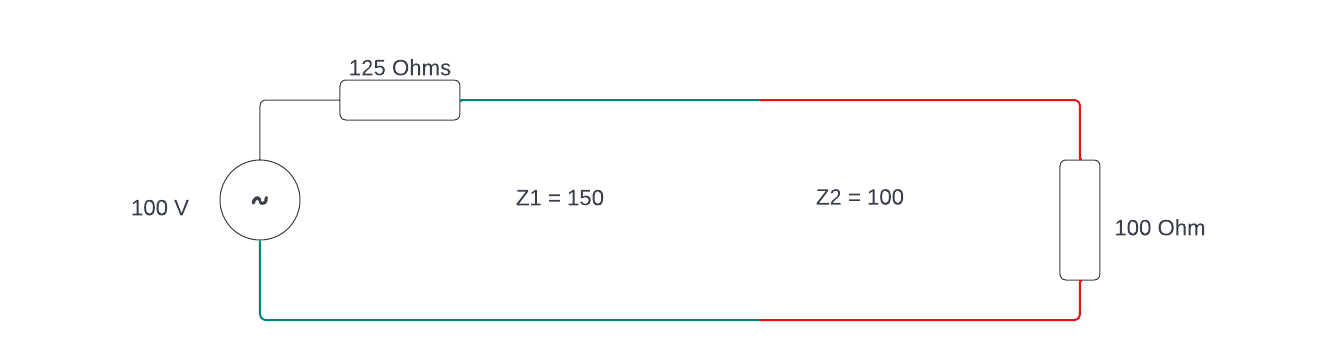
\includegraphics[width=
    \textwidth]{figures/Multiline_Example.png}
\end{center}
\end{figure}

Assume $f = 3$Mhz, speed of propagation at that frequency through the first transmission line is $300 km/s$ and speed of propagation through the second transmission line is $600 km/s$. Also assume that each half of the transmission line has a length of 300m.

Draw a bounce diagram depicting what happens for the first 5 milliseconds, assuming nothing was excited beforehand.

\newpage

\section{Terrific Transforms}

\begin{figure}[H]
\begin{center}
    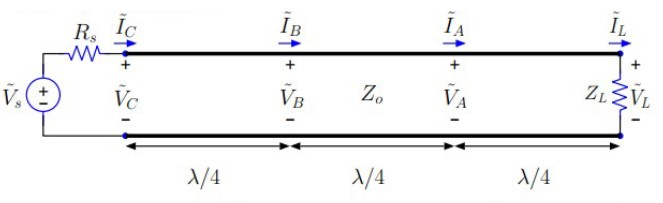
\includegraphics[width=0.93\textwidth]{figures/329 Problem 2.jpg}
\end{center}
\end{figure}

In the circuit above, $Z_0 = 50 \Omega$, $Z_L = 25 + j25 \Omega$, $R_s = 50 \Omega$, and $\tilde{V}_s = 20 V$. The line length if $3 \lambda / 4$. Answer the following questions:

\begin{enumerate}
    \item Determine impedance $\tilde{V}_B/\tilde{I}_B$ and explain. \vfill
    \item Determine impedance $\tilde{V}_C/\tilde{I}_C$ and explain. \vfill
    \item Use voltage division to determine voltage $\tilde{V}_C$ and show work. \vfill
    \item Determine $\tilde{V}_A$ and explain. \vfill
    \item Determine $\tilde{I}_L$ using the ``current forcing formula'' from $\tilde{V}_A$. \vfill
    \item Determine the average power absorbed in $Z_L$. \vfill
    \item Determine $\tilde{I}_B$ and explain. \vfill
\end{enumerate}

\newpage

\section{Sly Smith Charts}
\label{section:smith_chart}

The following is a series of conceptual questions meant to poke and prod at your understanding of Smith Charts.

\subsection{Magnificent Motivation}

Why do we use Smith Charts? What's wrong with our easy quarter-wave and half-wave transformers?

\vspace{3cm}

\subsection{Formal Formulae}
\label{section:formal_formulae}

Consider a TL with intrinsic impedance $Z_0$ and arbitrary length $l$ terminated by an arbitrary load $Z_L = R_L + jX_L$.

What is the equation for the voltage and current on the line at some arbitrary distance $d$ from the load in terms of the forward-going voltage $V^+$, the backward-going voltage $V^-$, the wave number $\beta$, and the intrinsic impedance of the TL $Z_0$?

\vspace{3cm}

\subsection{Realistic Reflections}
\label{section:realistic_reflections}

Now let us define the load reflection coefficient to be $\Gamma_L = \frac{Z_L - Z_0}{Z_L + Z_0}$. This should look familiar - it has a very similar form to the reflection coefficients from waves hitting a boundary!

Rewrite your answers from Section \ref{section:formal_formulae} in terms of $V^+$, $\Gamma_L$, $\beta$ and $Z_0$.

\vspace{3cm}

\subsection{Redefining Reflections}
\label{section:redefining_reflections}

Let's define a generalized reflection coefficient to be $\Gamma(d) = \Gamma_L e^{-j2 \beta d}$.

Rewrite your answers in Section \ref{section:realistic_reflections} in terms of $V^+$, $\Gamma(d)$, $\beta$, and $Z_0$. Also explain the significance of $\Gamma(d)$ - what does it mean when someone says $\Gamma(3) = 0.5$? What ranges of values can $\Gamma(d)$ take?

One important property of $\Gamma(d)$ is that it has a constant magnitude $\Gamma_L$ for all $d$ - only the phase changes. How is this represented on the Smith Chart?

\vspace{3cm}

\subsection{Intuitive Impedance}

Impedance, as a concept, is usually seen as voltage over current. Thus, take the equation for $V(d)$ that you found in \ref{section:redefining_reflections} and divide it by the equation for $I(d)$. Let's call this $Z(d)$. What is $Z(d)$?

\vspace{1cm}

\subsection{Quality Question}

A fellow student protests - "I thought the ratio between the voltage and current on the transmission line was always the intrinsic impedance of the transmission line, namely $Z_0$!"

Is the student wrong? Justify your answer.

\vspace{5cm}

\subsection{Noble Normalizations}

We find it convenient to normalize $Z(d)$, since we would like to generalize our example to transmission lines of any $Z_0$, not just a specific $Z_0$. Therefore, we define $z(d) = \frac{Z(d)}{Z_0}$.

We would also like to rewrite $\Gamma(d)$ in terms of $Z(d)$ and $Z_0$, for reasons we'll see later.

We also are going to stop writing $(d)$ everywhere because it is clear that these are functions of $d$.

Find $z(d)$ in terms of $\Gamma$ and find $\Gamma$ in terms of $Z$ and $Z_0$.

\vspace{3cm}

\subsection{Interesting Intermission}

This nice-looking relationship between $\Gamma$ and $z$ is known as a bilinear transformation, where bilinear refers to the fact that the numerator as well as the denominator of these transformations are linear with respect to the variable being transformed.

If you've taken ECE310 or are in it right now, then this is not the first bilinear transformation you've seen. The Laplace Transform and the z-transform also have a bilinear transformation between them, namely

$$H(z) = H_L(s) \vert_{s = \alpha \frac{1 - z^{-1}}{1+z^{-1}}}$$

Indeed, these two transformations are closely linked - their stability and causality conditions all map from one domain to the other flawlessly. And yes, the general shape of the transformation looks very similar to the Smith Chart.

More details of this can be found in MATH446 - Applied Complex Variables. But alas, I digress. Back to Smith Charts.

\subsection{Synthetic Shapes}

What are the lines on the Smith Chart that denote constant $r$ and constant $x$, where $z = r + jx$? Why do they look so weird and all over the place?

We define the normalized line admittance to be $y(d) = y = \frac{1}{z}$. Given a $z$ on the Smith Chart, where is $y$? Why?

\vspace{5cm}

\subsection{Pivotal Points}

What does the origin of the Smith Chart correspond to in terms of $\Gamma$? What does the origin of the Smith Chart correspond to in terms of $z$? What does the origin of the Smith Chart correspond to in real life?

What does the leftmost point of the Smith Chart correspond to in terms of $\Gamma$? What does the leftmost point of the Smith Chart correspond to in terms of $z$? What does the leftmost point of the Smith Chart correspond to in real life?

What does the rightmost point of the Smith Chart correspond to in terms of $\Gamma$? What does the rightmost point of the Smith Chart correspond to in terms of $z$? What does the rightmost point of the Smith Chart correspond to in real life?

\newpage

\subsection{Devious Details}

Let's now go over some of the methods that you've probably used when dealing with Smith Charts. We'll see if you know why those methods actually work.

\begin{enumerate}
    \item Matthew tells you that at the load end of the transmission line he's at angle 0 on the Smith Chart. He then walks 3 meters toward the input and asks what angle we're at now. What information are you missing to solve this problem? Why is it important?
    \item Matthew restarts at the load and walks $\frac{\lambda}{2}$ distance towards the input. How many degrees did he walk through on the Smith Chart? Why?
    \item Matthew receives a transmission line problem with some load impedance and some intrinsic impedance. He first normalizes the load impedance, enters it on the Smith Chart, and then draws a constant gamma circle that passes through the origin and the point he drew. Why did he do each of these three steps?
    \item Matthew finds the input impedance of some transmission line setup. He enters it on the Smith Chart and finds the phase and magnitude of $\Gamma$ at that point. What is the significance of this $\Gamma$?
    \item When travelling towards the source Matthew always rotates clockwise along the Smith Chart. Why? If Matthew instead travels towards the load then which direction should he rotate?
    \item Does the Smith Chart give you steady state solutions, transient solutions, or both?
\end{enumerate}

\newpage

\section{Quintessential Quarter-Wave}

A quarter-wave transformer will be inserted on the transmission line shown below some distance $d$ away from the load. Find $d$ and the optimal intrinsic impedance of the line to be inserted $Z_q$ such that the load depicted is a perfect match.

\begin{figure}[h]
\begin{center}
    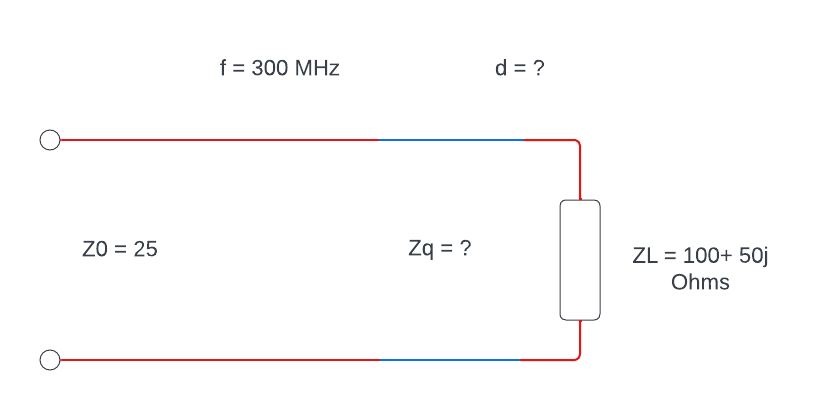
\includegraphics[width= 0.8
    \textwidth]{figures/Quarter_wave_transformer.png}
\end{center}
\end{figure}

Assume that $f = 300$MHz. Use a Smith Chart if you think you need one. Recall what you learned in Section \ref{section:smith_chart} and try and justify every step that you make.
\vfill

\newpage

\section{Vital VSWR}

Now that you have mastered Smith Charts, it's time to tackle the other difficult concept on the final - Voltage Standing Wave Ratio, or VSWR. Let's begin.

\subsection{Sedentary Standing Waves}

Here's a warmup question to get started - what is a standing wave?

\vspace{1cm}

\subsection{Monarchical Maxes and Mins}

Recall that $V(d) = V^+ e^{j \beta d} (1 + \Gamma_L e^{-j2\beta d})$ for any point on the transmission line that is a distance $d$ from the load, found earlier (if you do not remember why, go back and review! This is super important!)

What is the biggest value in magnitude that $V(d)$ can achieve? At what value of $d$ does this value appear? Note that we call this value of $d$ as $d_{max}$.

What is the smallest value in magnitude that $V(d)$ can achieve? At what value of $d$ does this value appear? Note that we call this value of $d$ as $d_{min}$.

For this problem assume that $\Gamma_L$ is a positive real number between and including 0 and 1.

\vspace{3cm}

\subsection{General Graphs}

Here is a graph that you may have seen before concerning $\vert V(d_{max}) \vert$ and $\vert V(d_{min}) \vert$. What is actually going on in the real world (in the time domain)?

\begin{figure}[h]
\begin{center}
    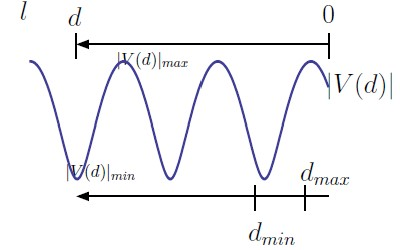
\includegraphics[width= 0.5
    \textwidth]{figures/Standing Wave Ratio.jpg}
\end{center}
\end{figure}

Hint: We have been almost exclusively dealing with what for half a semester?

Followup question: Does $z(d)$ or $\Gamma(d)$ depend on time? Why or why not?

\newpage

\subsection{Clever Convenience}

We want a standing wave ratio, so it seems logical that we should divide the maximum magnitude of $V(d)$ with the minimum magnitude of $V(d)$. Perform this calculation. Does the result seem familiar?

\vspace{4cm}

\subsection{Interesting Intermission 2}

Let's do a quick comparison.

$$VSWR = \frac{1 + \vert \Gamma_L \vert}{1 - \vert \Gamma_L \vert} \text{ and } \vert \Gamma_L \vert = \frac{VSWR - 1}{VSWR + 1}$$

$$z = \frac{1 + \Gamma}{1 - \Gamma} \text{ and } \Gamma = \frac{z - 1}{z + 1}$$

Yup. It's another bilinear transformation.

We note now that $\Gamma(d_{max}) = \vert \Gamma_L \vert$ (hopefully you saw this from the earlier parts). Therefore,

$$VSWR = \frac{1 + \vert \Gamma_L \vert}{1 - \vert \Gamma_L \vert} = \frac{1 + \Gamma(d_{max})}{1 - \Gamma(d_{max})}$$

So where is VSWR on the Smith Chart, and why is it where you specified?

\vspace{5cm}

\subsection{Electric Extremes}

What are the extreme values that VSWR can take on? What situations do they represent in real life?

\newpage

\section{Short and Stubby}

A transmission line with an intrinsic impedance of 300 $\Omega$ is connected to a load impedance of $450-j600$ and a signal with frequency $10$MHz. Find the position and length of a short-circuited stub required to match the line using a Smith Chart.

Don't just blindly apply the method you learned in class - instead think about why each step makes sense as you do it. There's no guarantee that the final exam will only contain simple impedance matching like what you learned in class.

\vfill

\section{Rebellious Resonance}

A lossless transmission line of length 600 meters is left open at $z = 0$ and shorted at $z = l = 600$m. Determine the resonant frequencies of the line.

\vfill

\newpage

\section{Daunting Distance}

\begin{figure}[H]
\begin{center}
    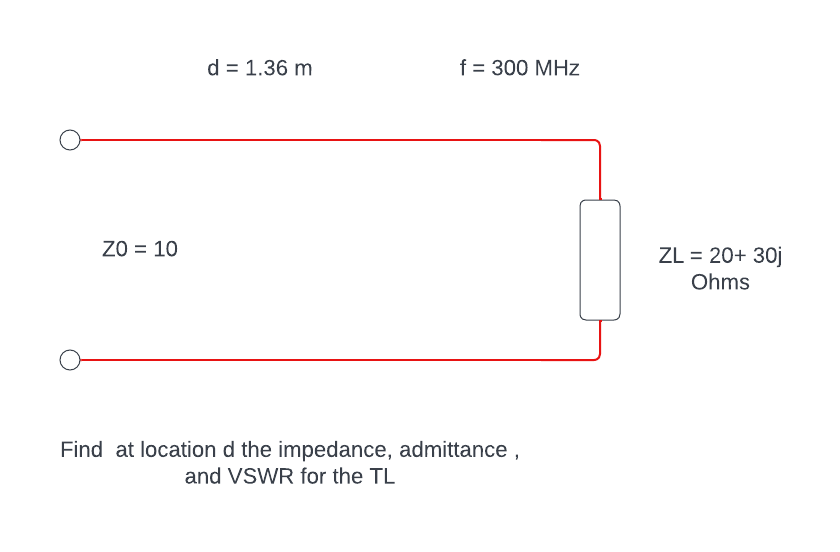
\includegraphics[width= 0.7
    \textwidth]{figures/VSWR Example.png}
\end{center}
\end{figure}

Assume that $f = 300$MHz. Also assume a velocity of $c$. Use a Smith Chart if you think you need one. Recall what you learned in Section \ref{section:smith_chart} and try and justify every step that you make.
\newpage


\section{Copious Coils}
A rectangular coil of dimensions a and b and resistance R moves with constant velocity v into a magnetic field as show below.

\begin{figure}[H]
\begin{center}
    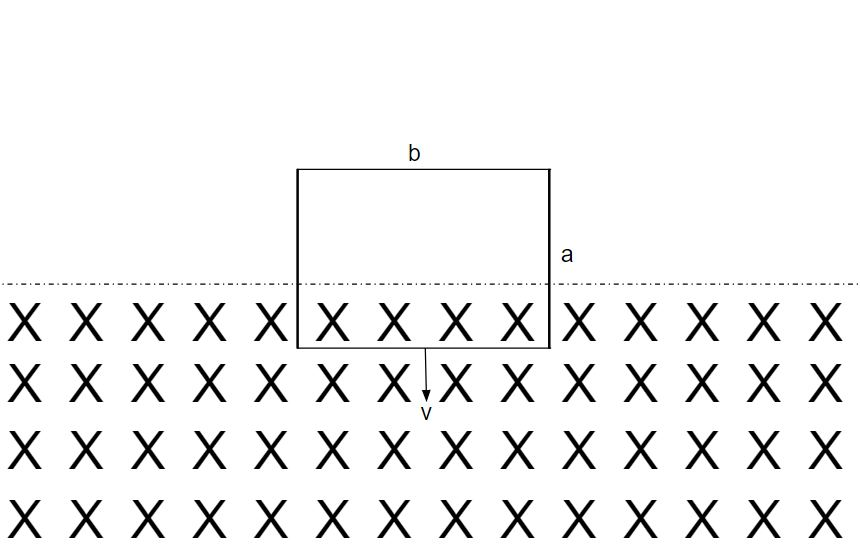
\includegraphics[width= 0.5\textwidth]{figures/square.jpg}
\end{center}
\end{figure}
\begin{enumerate}
    \item What is the emf induced in the coil? Express your answer in the appropriate units.
    \item What is the associated current? Express your answer in the appropriate units.
    \item What is the direction of the current flow?
\end{enumerate}
\vfill

\newpage

\section{Famous Fields}

In a homogenous medium, show that the phasor electric field in a source-free region satisfies the following relation, where $\beta$ is the wavenumber. DO NOT use your notes or textbook!

\[
\nabla^2 \tilde{E} + \beta^2\tilde{E} = 0
\]

Hint: $\nabla\times(\nabla\times \tilde{E}) = \nabla(\nabla \cdot \tilde{E}) - \nabla^2 \tilde{E}$.

\vfill

\section{Monumental Magnetics}

Consider an infinitely long conducting cylinder of radius $a$, with a cylindrical hole of radius $b$ placed at an offset $d$ from the center of the conductor. Assume that a static current $I$ is uniformly distributed across the cross-sectional area of the conductor. What is the magnetic field inside the hole?

\begin{figure}[H]
\begin{center}
    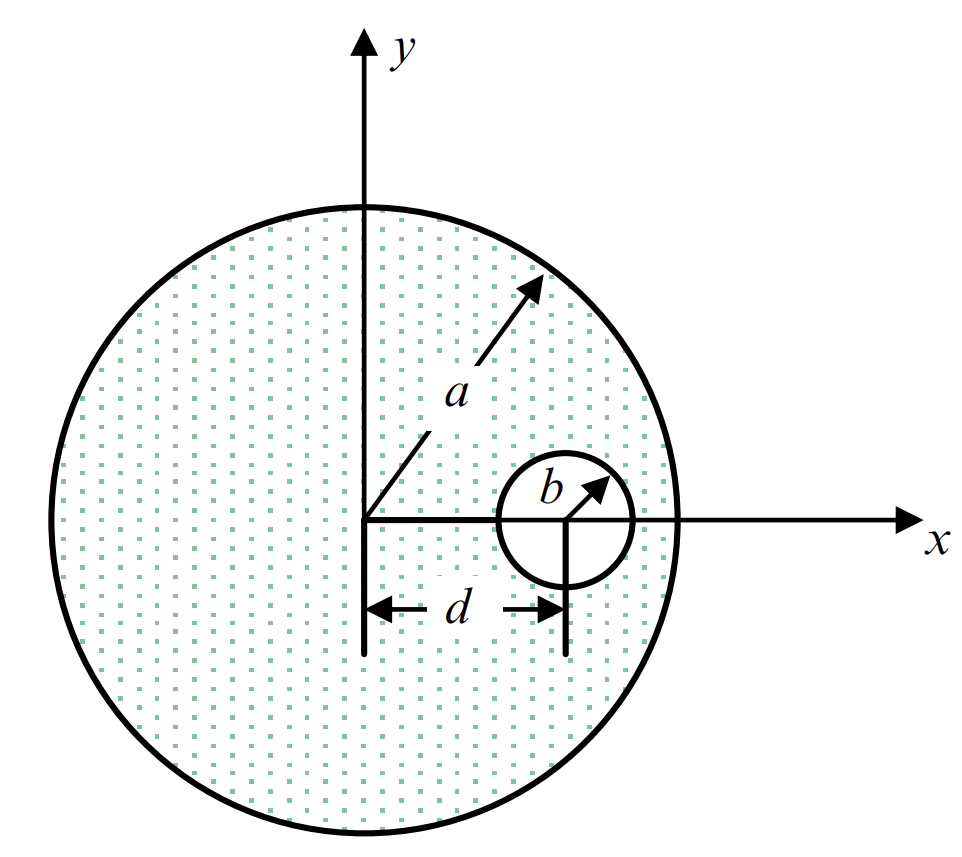
\includegraphics[width= 0.3\textwidth]{figures/cyl.png}
\end{center}
\end{figure}
\vfill
\newpage

\section{Deceptive Devices}

Consider the two devices below, with output and input impedances of 50 $\Omega$ and 200 $\Omega$ respectively. 

\begin{figure}[H]
\begin{center}
    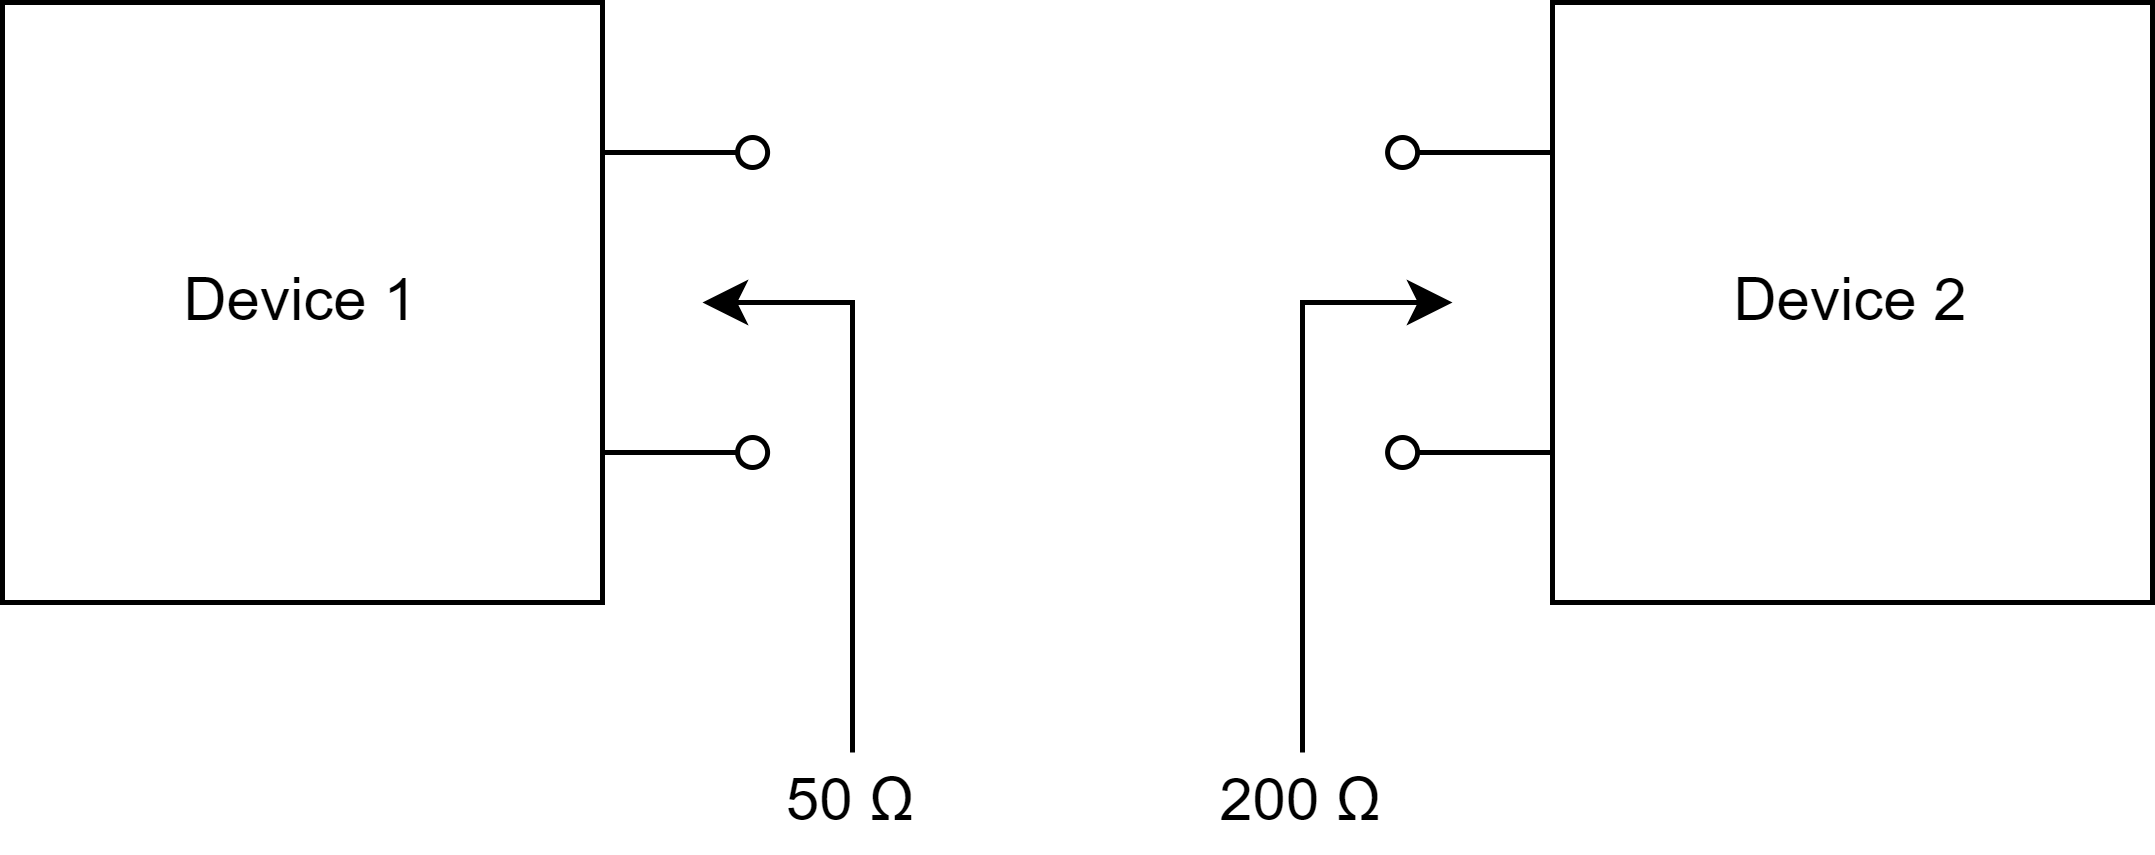
\includegraphics[width= 0.5\textwidth]{figures/matc.png}
\end{center}
\end{figure}

\subsection{Radical Reflections}
If we directly connect the two devices together, and device 1 outputs 30 dBm (1 Watt) of power at 1 MHz, how much power does device 2 receive?

\vfill

\subsection{Nefarious Networks}
Using a Smith Chart, design a L-matching network by first adding a shunt admittance, and then adding a series impedance, which will match the two devices at 1 MHz so that all of the power from device 1 is transferred to device 2. 
\vspace{3mm}

$\textbf{Hint 1:}$ Adding/subtracting reactance involves moving along the constant resistance circles.


\vspace{3mm}

$\textbf{Hint 2:}$ You should start by finding where 200 $\Omega$ falls on the admittance coordinates, and also drawing the $r = 1$ normalized admittance circle on the Smith Chart.

\vfill


\end{document}
